
In this chapter we give an algorithm for a relaxation of $\epsilon$-approximate hulls, called $(\epsilon, \delta)$ hulls. Our results hold for arbitrary point sets $P \subseteq \mathbb{R}^d$.
\\

Intuitively, an $(\epsilon,\delta)$ hull of $P$ is within distance $\epsilon$ from the boundary of the convex closure of $P$ in at least $1-\delta$ directions. We begin by giving an equivalent definition for an $\epsilon$-approximate convex hull, and then define $(\epsilon,\delta)$ hulls.

\section{Definition of $(\epsilon, \delta)$ hull}

\begin{definition}
Given a vector $v$ and a point set $P$, we define the \textbf{directional extent} as
\[ \omega_v(P) = \max_{p \in P} p \cdot v \]
\label{def:dir_extent}
\end{definition}
\begin{definition}
If $p$ is a point we define $\omega_v(p) = p \cdot v = \omega_v(\{p\})$
\end{definition}

It is easy to see that if $S \subseteq P$ then for all $v$, $\omega_v(S) \leq \omega_v(P)$.

\begin{definition}
We say $S$ \textbf{maximizes} $P$ in $v$ if
\[ \omega_v(P) = \omega_v(S) \]
Note that as per definition~\ref{def:dir_extent}, $S$ can be either a single vector or a set of vectors.
\end{definition}

\begin{figure}[!htb]
\centering
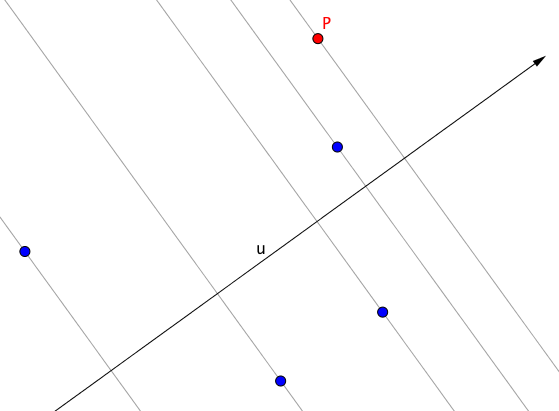
\includegraphics[width=0.5\linewidth]{maximal_point}
\caption{Point $p$ maximizes the set of points in direction $u$ because its projection onto $u$ is the highest.}
\label{fig:maximal_point}
\end{figure}

Figure~\ref{fig:maximal_point} shows a point $p$ that maximizes a set of points in direction $u$.

\begin{definition}
A \textbf{convex hull} is a subset $S \subseteq P$ such that $S$ maximizes $P$ in all (unit) directions $v$. 
\end{definition}

\begin{definition}
We say $S$ \textbf{$\epsilon$-maximizes} $P$ in direction $v$ if $v$ \emph{is a unit vector} and
\[ |\omega_v(P) - \omega_v(S)| \leq \epsilon \]
Note that as per definition~\ref{def:dir_extent}, $S$ can be either a single vector or a set of vectors.
\end{definition}

\begin{definition}
An \textbf{$\epsilon$-approximate convex hull} is a subset $S \subseteq P$ such that $S$ $\epsilon$-maximizes $P$ in all (unit) directions $v$. As before, OPT$(P, \epsilon)$ is the size of a smallest $\epsilon$-approximate convex hull.
\end{definition}

Intuitively, an $\epsilon$-approximate convex hull approximates the original point set in all directions. Coming up with a streaming algorithm that is competitive within a constant factor of OPT for this problem appears to be difficult. An interesting relaxation is to have a good approximation in \emph{most directions}. In the sections that follow, we will assume that the algorithm has access to OPT and sets $k = \mbox{OPT}$. In practice, we do not know OPT so we would simply set $k$ to be the largest value our computational resources permit. We would then have an $(\epsilon, \delta)$-approximation for all point sets where $\mbox{OPT} \leq k$. This is similar to the form of the lower bound we gave in theorem~\ref{thm:almostalwaysopt} in chapter~\ref{chapter:lower_bounds}.

\begin{definition}
An \textbf{$(\epsilon, \delta)$-hull} is the minimal sized set $S \subseteq P$ such that if we pick a vector $v$ uniformly at random from the surface of the unit sphere, $\mathcal{S}^{d-1}$, $S$ $\epsilon$-maximizes $P$ in direction $v$ with probability at least $1-\delta$, that is,
\[ \mbox{Pr}(|\omega_v(P) - \omega_v(S)| > \epsilon) \leq \delta \]
\end{definition}

Our goal is to come up with streaming algorithms for $(\epsilon, \delta)$-hulls that are competitive with OPT (the batch optimal for $\epsilon$-approximate convex hulls).

\section{Core Lemmas}

\begin{definition}
Define $E^S_s$ to be the set of all vectors $v$ in $\mathbb{R}^d$ (\emph{not just unit vectors}) such that $s$ maximizes $S$ in $v$, that is,
\[ E^S_s = \{ v \; | \; v \cdot s = \omega_v(S) \} \]
\end{definition}

\begin{figure}[!htb]
\centering
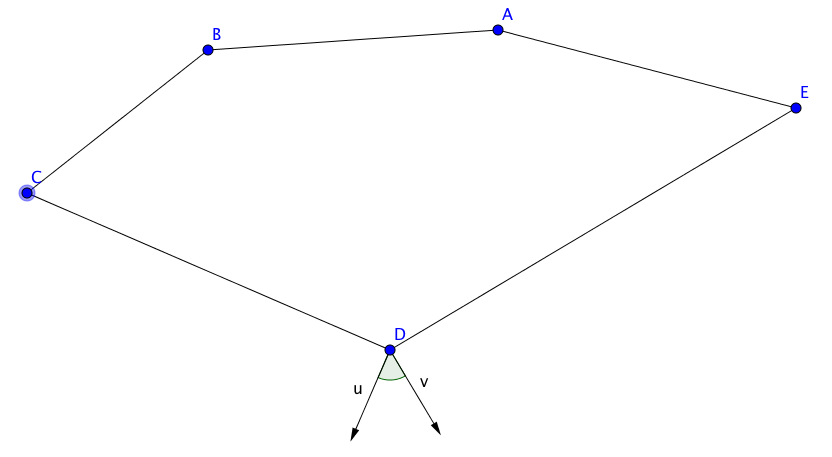
\includegraphics[width=0.7\linewidth]{maximizing_vector_range}
\caption{All vectors between $u$ and $v$ (not just unit vectors) are in $E_D^S$}
\label{fig:maximizing_vector_range}
\end{figure}

Figure~\ref{fig:maximizing_vector_range} shows a set of points $S$. All vectors between $u$ and $v$ (not just unit vectors), in the range indicated by the angle, are in $E_D^S$. Note that $u$ is perpendicular to line segment $CD$ and $v$ is perpendicular to line segment $DE$. Only points $s \in S$ that lie on the boundary of the convex closure of $S$ have non-empty $E_s^S$.

\begin{lemma}[$\epsilon$-Maximization Lemma] Suppose $S \subseteq P$ is an $\epsilon$-approximate convex hull of $P$, and fix $s \in S$. Then $s$ $\epsilon$-maximizes P for all unit vectors $v \in E^S_s$.
\end{lemma}

\begin{proof}
This is because for all unit vectors $v$, $|\omega_v(S) - \omega_v(P)| \leq \epsilon$ and for all vectors $v \in E^S_s$, $v \cdot s = \omega_v(S)$, so for all unit vectors $v \in E^S_s$, both properties hold.
\end{proof}

\begin{lemma}[Covering Lemma] For all vectors $v \in \mathbb{R}^d$,
\[ v \in \bigcup_{s \in S} E^S_s \]
\end{lemma}

\begin{proof}
Given any vector $v$, set $s = \displaystyle\argmax_{s' \in S} s' \cdot v$. Then $v \in E^S_s$.
\end{proof}

\begin{lemma} [Conic Lemma] $E^S_s$ is a cone, that is,
\begin{enumerate}
\item $0 \in E^S_s$
\item If $v \in E^S_s$ and $\alpha \in \mathbb{R^+}$ then $\alpha v \in E^S_s$.
\item If $v, w \in E^S_s$ then $v + w \in E^S_s$.
\end{enumerate}
\end{lemma}

\begin{proof} We prove each item,
\begin{enumerate}
\item $0 \cdot s = \max_{s' \in S} 0 \cdot s' = 0$
\item $(\alpha v) \cdot s = \alpha (v \cdot s) = \alpha (\max_{s' \in S} v \cdot s') = \max_{s' \in S} (\alpha v) \cdot s'$
\item $(v + w) \cdot s = (v \cdot s) + (w \cdot s) = \max_{s' \in S} v \cdot s' + \max_{s' \in S} w \cdot s' \geq \max_{s' \in S} (v + w) \cdot s'$
\end{enumerate}
\end{proof}

\begin{lemma} [Cutting Lemma] Given any 2 points $a \neq b \in \mathbb{R}^d$, let $H = \{v \; | \; v \cdot a \geq v \cdot b\}$. Then $H$ is a closed halfspace cutting through the origin.
\end{lemma}

\begin{proof}
Writing this in another way, $H = \{v \; | \; v \cdot (a - b) \geq 0\}$, which, if $a-b \neq 0$, is precisely the equation of a closed halfspace. The plane defining the boundary of the halfspace is defined by $P = \{v \; | \; v \cdot (a - b) = 0\}$ (that is, the set of all vectors perpendicular to $a-b$) which cuts through the origin.
\end{proof}

\begin{lemma} [Bounded Maximization Lemma] Suppose $S$ has at least 2 distinct points. Then if $s \in S$, $E^S_s$ is contained inside a closed halfspace passing through the origin.
\end{lemma}

\begin{proof}
Choose $s' \in S$ with $s' \neq s$. Then, let $H = \{v \; | \; v \cdot s \geq v \cdot s'\}$. $E^S_s \subseteq H$ but by the cutting lemma, $H$ is a closed halfspace passing through the origin.
\end{proof}

\section{2D-Algorithm}

We give a deterministic algorithm that stores $O(\frac{k}{\delta})$ points and gives us an $(\epsilon, \delta)$-hull of a point set $P$, where $k$ is the batch optimal for the $\epsilon$-approximate convex hull of $P$.
\\

\begin{figure}[!htb]
\centering
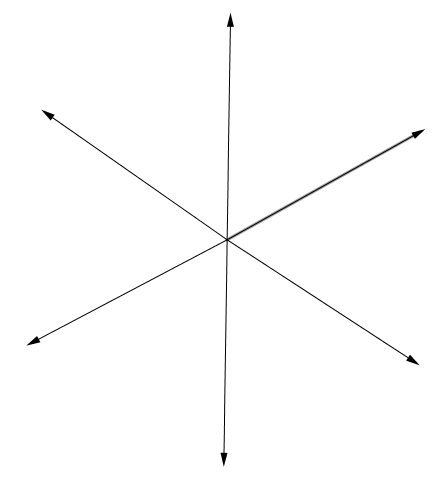
\includegraphics[width=0.3\linewidth]{equally_spaced_directions}
\caption{6 equally separated directions.}
\label{fig:equally_spaced_directions}
\end{figure}

Choose $O(\frac{k}{\delta})$ equally separated unit vectors (like in figure~\ref{fig:equally_spaced_directions}) on the boundary of the unit circle. Going counter-clockwise by angle, the angle formed by any 2 consecutive vectors will be less than $\frac{2\pi\delta}{k}$. For each chosen vector $v$ we store the point $p \in P$ s.t. $p \cdot v = \omega_v(P)$ ($p$ maximizes $P$ in $v$). This can be done in streaming - for a vector $v$, we keep an incoming point $p$ iff $v \cdot p$ is greater than $v \cdot p'$ for the point $p'$ we currently stored in direction $v$ (or if we have not stored any point for direction $v$). Call the set of points our algorithm chooses $T$.

\begin{theorem}
$T$ is an $(\epsilon, \delta)$-hull of $P$.
\end{theorem}

\begin{proof}
WLOG suppose that $P$ has at least 2 distinct points (otherwise we can trivially solve the problem by storing the only point in $P$). Consider an optimal $\epsilon$-approximate convex hull $S \subseteq P$. WLOG suppose that S contains at least 2 points (otherwise we can simply add some point in $P$ to $S$ and our bounds will only change by a constant factor). 
\\

\textbf{Partitioning}: Pick a vector $v$ uniformly at random on the boundary of the unit circle. By the covering lemma, $v \in E^S_s$ for some $s \in S$. Fix $s \in S$. It suffices to show the probability that $v \in E^S_s$ and $T$ does not $\epsilon$-maximize $P$ in direction $v$ is $\leq \frac{\delta}{k}$. Then, since there are $k$ choices for $s$, the probability $T$ does not $\epsilon$-approximate $P$ is $\leq k\frac{\delta}{k} = \delta$.
\\

\textbf{Angular setup}: Fix $s \in S$. $S$ has at least 2 distinct points, so by the cutting lemma, $E^S_s$ is contained in a half-space. So we can rotate space such that $E^S_s$ does not contain the positive x axis. We measure angles counter-clockwise from the positive x-axis. From the conic lemma, we know that $E^S_s$ is the set of all vectors with angles between $\theta_a$ and $\theta_b$ with $\theta_a < \theta_b$. Out of the $O(\frac{k}{\delta})$ vectors we chose, consider the subset of vectors that are in $E^S_s$. Call them $v_1, v_2, ..., v_m$ and suppose they have corresponding angles $\theta_1 < \theta_2 < ... < \theta_m$. We also have that $\theta_a \leq \theta_1$ and $\theta_m \leq \theta_b$.
\\

\begin{lemma}
Consider some $v_i$. We choose a point $p_i$ s.t. $p_i \cdot v_i = \omega_{v_i}(P)$ (that is, $p_i$ is maximal in direction $v_i$). We will show that $p_i$ $\epsilon$-maximizes either all unit vectors with angles in the range $[\theta_a, \theta_i]$ or in $[\theta_i, \theta_b]$
\end{lemma}

\begin{proof}
If $p_i = s$, then $p_i$ $\epsilon$-maximizes all unit directions in $E^S_s$, so we are done. Otherwise, suppose $p_i \neq s$. By the cutting lemma, there exists a closed half-space $H$ passing through the origin, such that $p \cdot v \geq s \cdot v$ iff $v \in H$. By the $\epsilon$-maximization lemma, for all unit vectors $v \in E_s$, $0 \leq \omega_v(P) - s \cdot v \leq \epsilon$. This implies that for all unit vectors $v \in E_s \cap H$, $0 \leq \omega_v(P) - p \cdot v \leq \omega_v(P) - s \cdot v \leq \epsilon$. In other words, $p$ $\epsilon$-maximizes all unit vectors $v \in E_s \cap H$.
\\

Since $E_s$ is itself contained in some halfspace passing through the origin, $E_s \cap H$ is either the set of vectors with angles in range $[\theta, \theta_b]$ or in range $[\theta_a, \theta]$. We note that $v_i \in E_s \cap H$ and has angle $\theta_i$, so in either case the range contains $\theta_i$. This proves the lemma.
\end{proof}

We say that $v_i$ is \emph{down} if $p_i$ $\epsilon$-maximizes $P$ in all directions with angles in the range $[\theta_a, \theta_i]$ and \emph{up} if $p_i$ $\epsilon$-maximizes $P$ in all directions with angles in the range $[\theta_i, \theta_b]$. If $v_1$ is up, then $p_1$ $\epsilon$-maximizes $P$ in all directions with angles in $[\theta_1, \theta_b]$. The angle between $\theta_a$ and $\theta_1$ is $\leq \frac{2\pi\delta}{k}$ because we chose vectors that were $\frac{2\pi\delta}{k}$ apart, so we are done. A similar argument applies if $v_m$ is down, and if $m = 0$ (we did not choose any vectors between $\theta_a$ and $\theta_b$. Otherwise, we consider the smallest $i$ s.t. $v_i$ is down but $v_{i+1}$ is up. Then, $p_i$ $\epsilon$-maximizes $P$ in all directions with angles in $[\theta_a, \theta_i]$ and $p_{i+1}$ $\epsilon$-maximizes $P$ in all directions with angles in $[\theta_{i+1}, \theta_b]$. We might not $\epsilon$-maximize $P$ in directions with angles in the range $[\theta_i, \theta_{i+1}]$, but this angle is $\leq \frac{2\pi\delta}{k}$.
\end{proof}


\section{Generalizing to higher dimensions}

\subsection{Algorithm}

Suppose we fix the dimension $d$. We give a randomized algorithm that uses $n$ points and with probability at least $1-p$ gives us an $(\epsilon, \delta)$-hull of a point set $P$, where $k$ is the batch optimal for the $\epsilon$-approximate convex hull of $P$ and $n$ satisfies,
\[ n \in O\left(\frac{k^2}{\delta^2}\left(\log{k} + \log{\frac{1}{\delta} + \log{\frac{1}{p}} }\right)\right) \]

Note that the given complexity hides the dependency on $d$, so the actual complexity will be $O(f(d) \frac{k^2}{\delta^2}\left(\log{k} + \log{\frac{1}{\delta} + \log{\frac{1}{p}} }\right))$ for some function $f : \mathbb{N} \to \mathbb{N}$
\\

The algorithm is simple: Choose $n$ random vectors on the unit sphere. For each chosen vector $v$ we store the point $p$ that maximizes $P$ in direction $v$, that is, $p \cdot v = \omega_v(P)$. As in the 2D algorithm, this can be done in streaming.

\subsection{3D Proof Outline}

As before, WLOG suppose that $P$ has at least 2 distinct points (otherwise we can trivially solve the problem by storing the only point in $P$). Consider an optimal $\epsilon$-approximate convex hull $S \subseteq P$. WLOG suppose that S contains at least 2 points (otherwise we can simply add some point in $P$ to $S$ and our bounds will only change by a constant factor). 
\\

\textbf{Constructing small triangular cones}: A triangular cone is a cone defined by the non-negative sums of 3 vectors. First, we choose $c$ ``small" triangular cones, where $c$ is a large constant. Consider a triangle cone defined by unit vectors $v_1, v_2, v_3$. More precisely, we choose the cones so that $\max(|v_1 - v_2|_2, |v_2 - v_3|_2, |v_1 - v_3|_2) < 0.01$. We choose the cones so that they are disjoint, and they span $\mathbb{R}^d$, that is, every vector is in some cone.. Intuitively, we can construct these cones as follows: we start out with $2^d$ triangular cones that span $\mathbb{R}^d$. Then we can keep making the cones smaller (we can select a vector in the middle of each cone to split it up into 3 cones) until the cones satisfy the required condition. The number of cones is some function of the dimension $d$.
\\

\textbf{Cutting cones}: Consider a cone $C \cap E^S_s$. Intuitively, we are going to show that each time we choose a vector $v$, we cut away part of $C \cap E^S_s$ (for the part we cut off, we have an $\epsilon$-maximization). Consider each unit vector $v$ we choose in cone $C \cap E^S_s$, and corresponding point $p$ that maximizes $P$ in $v$. If $p = s$, then $p$ $\epsilon$-maximizes the whole cone $E^S_s$ so we are done. Otherwise, by the cutting lemma, there exists a closed half-space $H$ passing through the origin, such that $p \cdot v' \geq s \cdot v'$ iff $v' \in H$. As in the 2D proof, $p$ then $\epsilon$-maximizes all vectors in $E^S_s \cap H$ and therefore in $C \cap E^S_s \cap H$. So the region of $C \cap E^S_s$ that we might not have $\epsilon$-maximized is $C \cap E^S_s \cap H^c$. $C \cap E^S_s \cap H^c \subseteq C \cap E^S_s \cap (H^c \cup \{0\})$. $(H^c \cup \{0\})$ is a cone, and the intersection of cones is a cone, so  $C \cap E^S_s \cap (H^c \cup \{0\})$ is also a cone. Note that $v \in H$ and $v \neq 0$, so $v \not\in C \cap E^S_s \cap (H^c \cup \{0\})$.
\\

\textbf{Projection}: After choosing many vectors $v \in C \cap E^S_s$, we end up with a cone $C' \subseteq C \cap E^S_s$ where $C'$ does not contain any of the selected vectors $v$. We want to show that the area of $C' \cap \mathbb {S}^2$ is less than $\frac{\delta}{ck}$ fraction of the unit sphere's area. Then, adding over the $ck$ cones, the proportion of unit vectors we don't $\epsilon$-maximize in $P$ is at most $\delta$. The main trick will be to project this into a 2-dimensional problem. Suppose that (triangular) cone $C$ was defined by vectors $v_1, v_2, v_3$. Consider the plane $P$ containing the endpoints of $v_1, v_2, v_3$. We project $C \cap E^S_s \cap \mathbb {S}^2$ onto $P$, and similarly project all unit vectors we chose that are in $C \cap E^S_s \cap \mathbb {S}^2$ onto $P$, and project $C' \cap \mathbb {S}^2$ onto $P$. 
\\

\textbf{Reduced problem}: This gives us a simpler problem. Suppose we have convex polygon $C$ with area $A$, where we choose points in $C$ from a nearly uniform distribution $\pi$. More formally, the ratio between the max and min of the PDF of $\pi$ is at most 2. Call a convex polygon \emph{respectful} if it does not contain any selected points. How many points do we need to choose so that with high probability, all respectful convex polygons contained in $C$ must have area $\leq \frac{\delta}{k}$? The reason this reduction holds is because we chose cone $C$ to be small, so $C \cap \mathbb {S}^2$ is quite flat. In particular, if we rotate space so that plane $P$ is perpendicular to the $z$ axis, the norm of the gradient of $C \cap \mathbb {S}^2$ is bounded by 2. So when a set of measure $v$ in $C \cap E^S_s \cap \mathbb {S}^2$ is projected to $P$ it has measure between $\frac{v}{2}$ and $v$.

\begin{lemma}
Given a convex polygon $C$, there exists 3 points in $C$ such that the triangle formed between them has area at least $\frac{1}{4}$ the area of $C$.
\label{lemma:convex_approx}
\end{lemma}

\begin{lemma}
The pdf of $\pi$ must be between $\frac{1}{2A}$ and $\frac{2}{A}$ everywhere.
\end{lemma}

\textbf{Uniform Bound Outline} Let $T$ be the set of triangles contained in polygon $C$ with area $\geq \frac{\delta}{4ck}$.  Given $t \in T$, let $P(t)$ denote the probability that a point selected from $\pi$ lies in $t$. Since $\pi$ is almost uniform, $P(t) \geq \frac{\delta}{8Ack}$. We will use uniform bounds and VC dimension, to show that if we select enough points in $C$ then with high probability \emph{every} triangle in $T$ will contain a point. This is sufficient to solve the problem: consider arbitrary convex polygon $G$ contained in $C$ with area $\geq \frac{\delta}{ck}$. By lemma~\ref{lemma:convex_approx}, it contains a triangle of area $\geq \frac{\delta}{4ck}$. But all such triangles contain a point, so $G$ contains a point. Therefore every convex polygon in $C$ that does not contain a point must have area $< \frac{\delta}{ck}$.
\\

\textbf{Sampling Process} Select $n$ points in $C$ from distribution $\pi$. For $t \in T$, let $C_n(t)$ be the number of selected points that lie in $t$, and let $P_n(t)$ be $\frac{C_n(t)}{n}$. Intuitively, we are estimating the cumulative density of $\pi$ in a region by sampling points and computing the proportion of points that fall in the region. Suppose that for all $t \in T$, $|P_n(t) - P(t)| < \frac{\delta}{8Ack}$ (this means that $P_n$ approximates $P$ well). Then, for all $t$, since $P(t) \geq \frac{\delta}{8Ack}$, $P_n(t) > 0$. This means that every triangle $t \in T$ contains a point.
\\

\textbf{VC Dimension} We want to show that with probability at least $1-\frac{p}{2ck}$, $\sup_{t \in T} |P_n(t) - P(t)| < \frac{\delta}{8Ack}$. The VC dimension of $T$ is 7. Letting $\epsilon = \frac{\delta}{8Ack}$, we apply a VC-dimension based uniform bound to get that,
\[ P(\sup_{t \in T} |P_n(t) - P(t)| > \epsilon) \leq 8(n+1)^7 e^{-n\epsilon^2/32} \]

We set $n \in O(\frac{(Ack)^2}{\delta^2} (\log{\frac{Ack}{\delta}} + \log{\frac{k}{p}}))$.
\\

\textbf{Finishing up}: Consider a cone $C \cap E^S_s$. Suppose that the intersection $C \cap E^S_s \cap \mathbb {S}^2$ has area $A$. The projection has area $\leq A$, so it suffices to choose $n \in O(\frac{A^2k^2}{\delta^2} (\log{\frac{Ak}{\delta}} + \log{\frac{k}{p}}))$ unit vectors in $C \cap E^S_s \cap \mathbb {S}^2$. When we choose a unit vector at random, it lies in $C \cap E^S_s \cap \mathbb {S}^2$ with probability $c = \frac{A}{4\pi}$. We want to choose $m$ points, so that with probability at least $1-\frac{p}{2ck}$ we have $n$ points inside the cone. From a standard Chernoff bound argument, $m \in O(\frac{n}{c}(\log{n} + \log{\frac{k}{p}} ))$ works. Simplifying, this becomes,
\begin{align*}
m &= O\left(\left[\left(\frac{A^2k^2}{\delta^2} \left(\log{\frac{Ak}{\delta}} + \log{\frac{k}{p}}\right)\right)\left(\frac{4\pi}{A}\right)\right]\left[ \log{n} + \log{\frac{k}{p}} \right]\right) \\
&= O\left( \left[\left(\frac{Ak^2}{\delta^2} \left(\log{\frac{Ak}{\delta}} + \log{\frac{k}{p}}\right)\right)\right]\left[ \log{n} + \log{\frac{k}{p}} \right] \right)
\end{align*}

We note that $A \leq 4\pi$. Furthermore, $\log{n}$ actually simplifies to
\[ O(\log{\frac{k}{\delta}} + \log(\log{\frac{k}{\delta}} + \log{\frac{k}{p}})) \subseteq O(\log{\frac{k}{\delta}} + \log{\frac{k}{p}}) \]

So in the worst case $m$ reduces to
\[ m \in O\left(\frac{k^2}{\delta^2}\left(\log{k} + \log{\frac{1}{\delta} + \log{\frac{1}{p}} }\right)\right) \]
We can apply union bounds over the cones to get a $\leq p$ chance of failure.

\subsection{Arbitrary Dimension Proof Sketch}

A few parts of the proof need to be modified to deal with higher dimensions.
\begin{enumerate}
\item The section where we construct small triangular cones. In $d$ dimensional space, the cones will be defined by $d$ vectors (so the endpoints of the vectors form a simplex instead of a triangle) such that the pairwise distance between any 2 vectors is at most 0.1. The construction is as described above.
\item We need to modify lemma~\ref{lemma:convex_approx}. In particular instead of triangles, we will use ellipsoids. Given any convex body $C$ with area $A$, there exists an ellipsoid contained inside $C$ with area at least $A/d^d$~\cite{geom_approx_algs}.
\item The VC dimension of an ellipsoid in $d$-dimensional space is $O(d^2)$ (we used the factor that the VC dimension of a triangle in 2D space is 7).
\end{enumerate}
The rest of the proof outline is the same, so this gives us the desired result.